\documentclass[a4paper,10pt]{article}

\usepackage{fullpage}
\usepackage[T1]{fontenc}
\usepackage{graphicx}
\usepackage{float}
\usepackage{amsmath}
\usepackage{tabulary}
\usepackage{listings}
\usepackage[spanish]{babel}
\usepackage[utf8]{inputenc}
\usepackage{color}
\usepackage[pdfborder={0 0 0}]{hyperref}
\usepackage{alltt}
\usepackage{moreverb}
\usepackage{enumitem}
\usepackage{array}



% Título principal del documento.`
\begin{document}
\title{	
	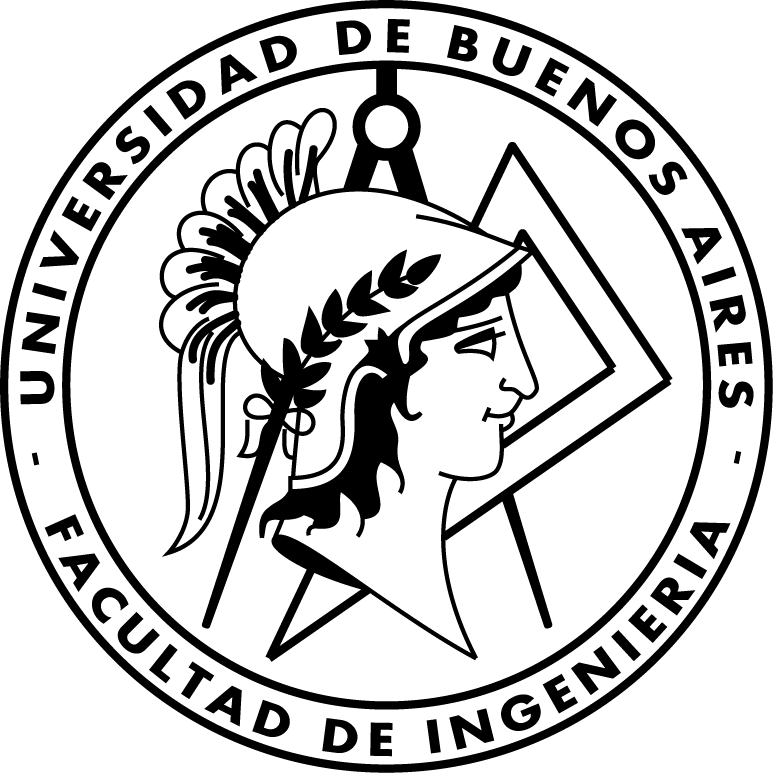
\includegraphics[scale=0.8]{images/logo-fiuba.png} \\
	\begin{center}
		\textbf{Trabajo Práctico N$^{\circ}$2} \linebreak
	\end{center}
	\begin{center}
		\begin{large}
			75.29 - Teoría de Algoritmos I \linebreak
			Facultad de Ingeniería de la Universidad de Buenos Aires \linebreak
			1er. Cuatrimestre 2017 \linebreak
		\end{large}
	\end{center} 
}
\author{	Federico Brasburg, \textit{Padrón Nro. 96.653} \\
			\texttt{ federico.brasburg.@gmail.com } \\ [2.5ex]
			Pablo Rodrigo Ciruzzi, \textit{Padrón Nro. 95.748} \\
			\texttt{ p.ciruzzi@hotmail.com } \\ [2.5ex]
			Andrés Otero, \textit{Padrón Nro. 96.604 } \\
			\texttt{ oteroandres95@gmail.com } \\ [2.5ex] \\
\\
		}
\date{5 de junio de 2017}

\maketitle
\thispagestyle{empty}

\pagebreak 

\tableofcontents
\pagebreak

\clearpage
\section{Clases de Complejidad}

\subsection{Punto 1}
	Es un problema que tiene un algoritmo que lo resuelve de manera óptima en tiempo polinomial. Dicho algoritmo es del tipo greedy y es el siguiente:
	\lstset{
		mathescape, columns=fullflexible, basicstyle=\fontfamily{lmvtt}\selectfont,
	}
	\begin{lstlisting}
	def actividades_compatibles(actividades):
	    ordenar actividades por tiempo de finalizacion en orden creciente
	    inicializar S con la primer actividad (la que tiene el fin mas chico)
	    para cada actividad A en la lista ordenada de actividades:
	        si A.principio $\geq$ S[ultimaActividadAgregada].fin entonces:
	            agregar A a S
	    devolver S
	\end{lstlisting}

	El algoritmo es $O(n.log(n))$ en tiempo debido al ordenar. Este algoritmo devuelve cuales actividades que hacen máxima la cantidad de actividades que se realizan; basta con contarlas y ver si es mayor o igual a $k$ para dar respuesta al problema original.

\subsection{Punto 2} \label{punto2}
	Es un problema NP-Completo. Para demostrar esto, primero mostramos que está en NP. Un problema está en NP si existe un algoritmo de orden polinomial que, a través de una instancia y un certificado, responda si el certificado da respuesta a la instancia del problema. En este problema siendo la instancia del problema todas las actividades posibles (y sus tiempos) y el certificado el conjunto de actividades compatibles, el algoritmo es trivial, ya que basta con ver que las actividades del certificado sean compatibles y que la cantidad de actividades sea mayor o igual a k.

	Ahora hay que encontrar un algoritmo X tal que $X \leq Problema2$ (siendo $\leq$ un operador polinomial, y Problema2, el problema de este ejercicio). Esto es, encontrar X de manera de poder reducirlo polinomialmente a Problema2 para poder decir ``X no es más difícil que Problema2'' y si X es de los llamados “difíciles” entonces Problema2 también lo será.

	El elegido como problema ``X'' es Set Packing, que es un problema NP-Completo clásico, en el cual existe un universo U, un conjunto de subconjuntos de $U$ que llamaremos $S$ y en el cual, dado un $k$, hay que ver si existe un subconjunto de $S$ de subconjuntos de $U$ de tamaño $k$ o mayor. La transformación polinómica que proponemos para llevar ese problema al problema que queremos demostrar es el siguiente:
	\begin{itemize}
		\item $k$ de Set Packing es igual al de las actividades.
		\item Transformamos los elementos de U en S a números mediante una función de hashing en un valor número entero.
		\item A cada subconjunto contenido en S lo pasamos a llamar tareas, resultando $T_1, T_2, ..., T_n$ tareas.
		\item Para elemento en cada $T_i$, creamos un intervalo en ese $T_i$, siendo el start el elemento y el end el elemento más uno, quedando así cada tarea con intervalos de duración 1.
		\item Le pasamos estas tareas y el $k$ a nuestro problema y la respuesta que dé nuestro problema va a ser la misma que la de Set Packing.
	\end{itemize}

	Entonces Problema2 es NP-Completo.

\subsection{Punto 3}
	Utilizando el método especificado en \ref{punto2}, pasamos a demostrar que el problema del camino Hamiltoniano es un problema NP-Completo:

	$\bullet$ Demostramos que está en NP

	Esto es trivial en el problema: dado un certificado que sería una secuencia de vértices del grafo simplemente hay que comprobar que existe una arista que va desde un determinado vértice al siguiente en la secuencia. Tomando en cuenta que la secuencia cuenta con todos los vértices, esta comprobación es de tiempo lineal. Expresado de manera formal sería:
	\emph{Dado  una secuencia (V\textsubscript{Inicial}, ...,V\textsubscript{Final}) de tamaño |V|, $\exists$ (V\textsubscript{i}, V\textsubscript{i+1}) $\in$ E $\forall$ i=1..N $\wedge$ $\exists$ (V\textsubscript{Final},V\textsubscript{Inicial}) $\in$ E } \\

	$\bullet$ Lo reducimos a un problema NP-Completo:

	Vamos a reducir el problema a 3-SAT usando un \textbf{``gadget''}.

	\texttt{3-SAT $\leq_p$ Hamilton}
	\linebreak

	El problema 3-SAT es: dado cláusulas booleanas de 3 variables que pueden ser verdad o no, vamos a resolver una instancia general de 3-SAT con una instancia particular del problema del camino Hamiltoniano.

	Dada una instancia de 3-SAT con variables $x_1, ..., x_n$ y cláusulas $c_1, ..., c_k$, podemos generar un digrafo que tenga $n$ caminos. Cada camino tiene $3k+3$ vértices y cada camino va en ambos sentidos. Además conectamos el primer y el último camino con el primero y el último del próximo camino. Finalmente agrego un nodo al principio que conecte con el primer y último nodo; también conecto el primer y último nodo del último path con otro nodo y conecto este último con el conectado con el primero. Finalmente queda un grafo como se muestra en la figura \ref{fig:punto-3-1}.

	\begin{figure}[!htb]
		\centering
		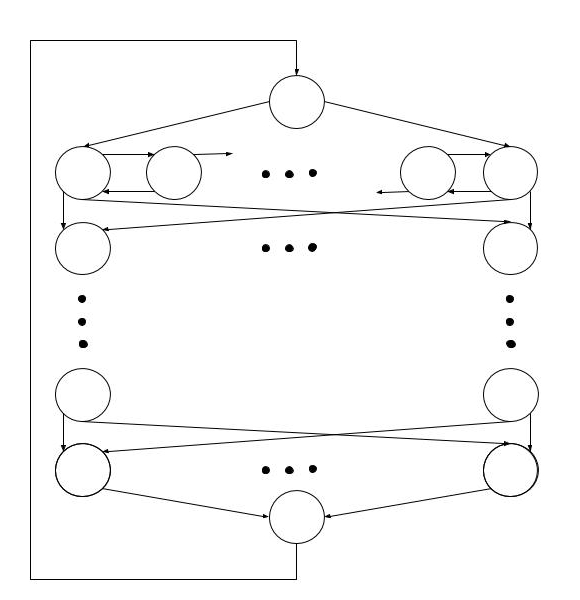
\includegraphics[scale=0.35]{images/grafo-3-1.jpg}
		\caption{Grafo resultante de la reducción de 3-SAT.}
		\label{fig:punto-3-1}
	\end{figure}

	De esta manera lo que estamos haciendo es replicando en un grafo que tiene $2n$ posibles ciclos hamiltonianos, las $2n$ posibles combinaciones de las $n$ variables booleanas. Lo podemos pensar como si el ciclo se recorre de izquierda a derecha, su variable análoga vale 1 y si es al revés vale 0.

	Teniendo esto en mente, podemos terminar de armar nuestro grafo utilizando un nodo más para simular una cláusula. Éstas van a estar conectadas a aristas en el mismo sentido que debe recorrer los caminos para que su variables den el valor asociado. Para clarificar, teniendo una cláusula h que tiene la forma $(x_1 \vee x_2 \vee x_3)$, se agrega un vértice $V_h$ que va a estar conectado a $V_{1,L}, V_{2,L+1}, V_{3,L}$ y aristas desde $V_{1,L+1}, V_{2,L}, V_{3,L+1}$. Para clarificar la notación $V_{1,L}$ es el vértice L de izquierda a derecha del primer camino. Ahora si $P_1$ recorre de izquierda a derecha puede visitar a $V_h$. Para hacerlo más general cada cláusula $C_j$ de variables $x, y, z$ estará conectado con $V_{x,3j}, V_{y,3j}, V_{z,3j}, V_{x,3j+1}, V_{y,3j+1}, V_{z,3j+1}$. De esta manera sabemos que una cláusula puede ser satisfecha si y sólo si una de sus variables toma el valor necesario, que es análogo a que es visitado si el camino asociado a la variable correspondiente es recorrido de manera correspondiente con el valor de esa variable. Quedando entonces un grafo similar al de la figura \ref{fig:punto-3-2}.

	\begin{figure}[!htb]
		\centering
		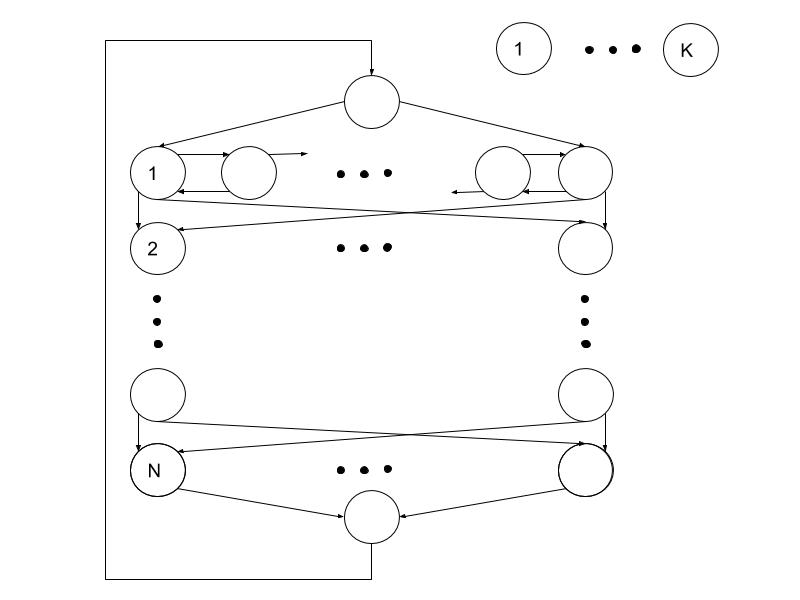
\includegraphics[scale=0.35]{images/grafo-3-2.jpg}
		\caption{Grafo final de la reducción de 3-SAT.}
		\label{fig:punto-3-2}
	\end{figure}

	Para finalizar podemos decir que el problema es satisfacible si y sólo si existe un ciclo hamiltoniano que lo cumpla, ya que las cláusulas serán visitadas (y solo pueden ser visitadas si se cumplen) si existe un camino hamiltoniano.

\subsection{Punto 4}
	Este problema es P y su algoritmo de resolución es bastante sencillo. Utilizando el algoritmo de orden topológico encontramos el orden lineal que conserva la unión entre vértices. Una vez que terminamos este ordenamiento, simplemente si todos los nodos se conectan con su siguiente entonces existe un camino hamiltoniano. La idea surgió de un ejercicio parecido hecho anteriormente.
	\begin{lstlisting}
	DAG_Hamiltoniano (grafo G):
	    lista = Ordenar_Topologicamente(G)
	    for i in |lista|-1:
	        if (lista[i],lista[i+1]) $\notin$ E[G]:
	            return False
	    return True
	Ordenar_Topologicamente (grafo G):
	    lista=[]
	    for each vertice u $\in$ V[G]:
	        estado[u] = NO_VISITADO
	        padre[u] = NULL
	    tiempo = 0
	    for each vertice u $\in$ V[G]:
	        if estado[u] = NO_VISITADO:
	            Visitar(u)
	    return lista
	Visitar(nodo u)
	    estado[u] = VISITADO
	    tiempo = tiempo + 1
	    distancia[u] = tiempo
	    for each v $\in$ Adyacencia[u]:
	        if estado[v] = NO_VISITADO:
	            padre[v] = u
	            Visitar(v)
	    estado[u] = TERMINADO
	    tiempo = tiempo + 1
	    finalizacion[u] = tiempo
	    list.add(u)
	\end{lstlisting}

\subsection{Punto 5}
	El problema de búsqueda de ciclos negativos es posible de resolver en forma polinómica. Generalmente, algunos algoritmos de grafos cuya intención primera no es encontrar ciclos negativos, tienen la funcionalidad de encontrarlos como un ``beneficio'' adicional. Un ejemplo conocido es el algoritmo de Bellman-Ford, cuyo objetivo es encontrar, dado un origen, caminos mínimos a todos los nodos de un grafo, aún para grafos con aristas con peso negativo. A continuación mostramos dicho algoritmo, y cómo hace para detectar los ciclos negativos en tiempo polinomial:
	\begin{lstlisting}
	Bellman-Ford(G, s):
	$\forall$ v $\in$ G.vertices:
	    v.dist = $\infty$
	s.dist = 0
	$\forall$ i = 1..|G.vertices| - 1:
	    $\forall$ a=(u,v) $\in$ G.aristas:
	        if v.dist $>$ u.dist + d(u,v)
	            v.dist = u.dist + d(u,v)
	\end{lstlisting}

	Una vez finalizado este simple algoritmo (Que tiene tiempo $O(|V|.|A|)$, es decir, polinomial), con la información obtenida, se puede hacer la detección de ciclos negativos, donde se devolvería verdadero o falso indicando si hay o no un ciclo negativo:
	\begin{lstlisting}
	$\forall$ a=(u,v) $\in$ G.aristas:
	    if v.dist $>$ u.dist + d(u,v)
	        return true
	return false
	\end{lstlisting}

\subsection{Punto 6}
	Este problema se puede comprobar que es un problema NP-Completo, así como se describió en \ref{punto2}. Para ello, basta con comprobar las 2 condiciones necesarias para dicha condición:

	$\bullet$ El problema es NP

	Esto es relativamente simple. Básicamente, recibiendo una instancia (un grafo) y un certificado (Un conjunto de vértices y aristas indicando el ciclo), habría que comprobar que es un ciclo (Lo cual se puede comprobar en $O(|V|+|A|))$ y que la suma de los pesos de las aristas es 0.
	\linebreak

	$\bullet$ El problema es NP-Hard

	Para esto, se utiliza algún problema NP-Completo de tal manera que, reduciendo ese problema al nuestro en tiempo polinomial, se demuestra que nuestro problema es al menos tan difícil que dicho problema NP-Completo. En este caso, el problema NPC a utilizar va a ser Subset Sum, ya que por su naturaleza (Ver si dentro de un conjunto de números hay un subconjunto cuya suma es igual a 0), parecería una buena elección para nuestro problema. Entonces, hay que encontrar una transformación polinómica para demostrar que:

	\texttt{Subset Sum $\leq_p$ ZWC (Zero Weight Cycle)}
	\linebreak

	La idea de la reducción es, dado un conjunto $S={x_1, x_2, ..., x_n}$ de números, generar un grafo completo de $n$ vértices, donde a cada vértice $i$, desde cada uno de los otros, entre una arista con peso $x_i$. Así se puede asegurar que, al ser completo, siempre que exista un ciclo de peso 0, existirá un subconjunto $T \subseteq S$, cuya suma sea igual a 0. El único caso particular a tener en cuenta ya que traería problemas, es si dentro de $S$ se encuentra el número 0. En ese caso, la idea sería detectar antes de pasarlo al grafo y devolver directamente que existe el subconjunto con suma igual a 0 (Ya que sino no se detectaría el grafo con camino de peso igual a 0). Por último, cabe aclarar que dicha transformación es polinómica, ya que para generar el grafo completo dado el conjunto $S$, se requiere la creación de $n$ vértices y $n.(n-1)$ aristas. Es decir, la transformación es $O(n^2)$.

	Por ejemplo, dado el conjunto $S = \{5, 4, -2, -3\}$, el grafo y su respectiva solución sería el de la figura \ref{fig:punto-6}.

	\begin{figure}[!htb]
		\centering
		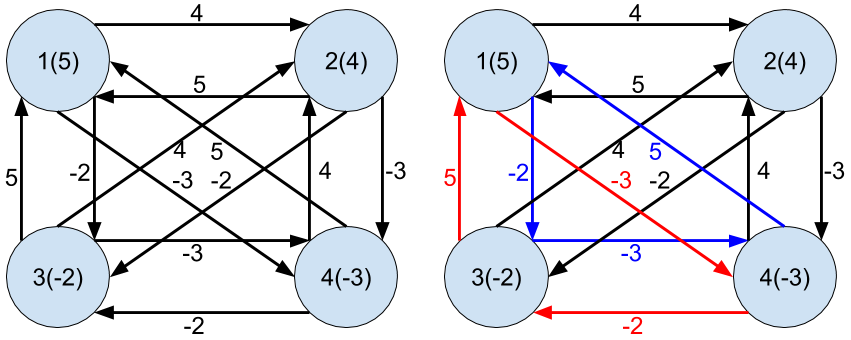
\includegraphics[scale=0.4]{images/grafo-6.png}
		\caption{Problema 6.}
		\label{fig:punto-6}
	\end{figure}

	Donde se puede observar que, como existe un subconjunto $\{5, -2, -3\}$ cuya suma es 0, existe al menos un ciclo en el grafo correspondiente.

\section{Algoritmos de camino mínimo}
\subsection{Dijkstra}
	Dijkstra funciona de manera Greedy, donde dado un origen busca en cada iteración el camino más corto a todos los nodos. Optimizado utilizando una estructura de tipo $heap$ para encontrar la menor distancia en cada paso, el algoritmo es $O(|A|+|V|.log(|V|))$.

\subsection{Bellman-Ford}
	El algoritmo de Bellman-Ford es un algoritmo de programación dinámica. Funciona análogamente al de Dijkstra pero en vez de buscar en cada iteración la arista de peso mínimo, relaja (es decir, recalcula la distancia para todos los nodos) en cada iteración todas las aristas, realizándolo para cada nodo. El tiempo de ejecución del algoritmo es $O(|A|.|V|)$.

\subsection{Floyd-Warshall}
	El objetivo de Floyd-Warshall es calcular todos los caminos mínimos entre todos los pares del grafo. Intuitivamente, uno pensaría hacer $|V|$ veces Bellman-Ford, lo cual resultaría en un algoritmo $O(|A|.|V|.|V|) \approx O(|V|^4)$. De todas formas, este algoritmo corre en $O(|V|^3)$. La idea es, utilizando una matriz de distancias, ir calculando el camino mínimo entre todos los pares, agregando en cada iteración la posibilidad de pasar por un vértice más. Este algoritmo se corresponde con la técnica de programación dinámica.

\subsection{Comparación}
	Como principales diferencias, podemos decir que Dijkstra no acepta aristas con pesos negativos, mientras que Bellman-Ford y Floyd-Warshall sí aceptan. Fuera de eso, el resultado de Dijkstra y Bellman-Ford debería ser el mismo, ya que resuelvan el mismo problema. Por otro lado, los tiempos de ejecución son distintos, siendo Dijkstra el de menor tiempo, y siendo Bellman-Ford y Floyd-Warshall del mismo de orden de magnitud. Por último, como ya se mencionó, Dijkstra y Bellman-Ford dan el resultado para un vértice de origen, mientras que Floyd-Warshall da los caminos mínimos para todo el grafo.

\subsection{Detección de ciclos negativos}
	Tal como se mencionó en el punto 5 de la primera parte del TP, se podría utilizar el algoritmo de Bellman-Ford para encontrar ciclos negativos.

	Por otro lado, Dijkstra no es capaz, ya que ni siquiera admite aristas con pesos negativos, por lo que un ciclo negativo sería imposible de detectar.

	En cuanto a Floyd-Warshall, también es capaz de identificar ciclos negativos. En este caso, el resultado devuelto por el algoritmo es incorrecto, y uno puede darse cuenta de dicha situación viendo que en la diagonal principal de la matriz hay valores negativos.

\subsection{Resultados}
	Habiendo generado 10 archivos con grafos completos con pesos positivos aleatorios entre 0 y 2, logramos correr los siguientes algoritmos en los tiempos indicados:

	\begin{center}
		\begin{tabular}{ |c|c|c|c|c|c| }
			\hline
			\textbf{Tamaño} & \textbf{Dijkstra} & \textbf{Bellman-Ford} & \textbf{Floyd-Warshall} & \textbf{Dijkstra Unitario} & \textbf{Bellman-Ford Unitario} \\ 
			\hline
			10 & 0,000026 & 0,003331 & 0,000353 & 3,10E-06 & 0,00045 \\ \hline
			20 & 0,000032 & 0,068222 & 0,002055 & 5,01E-06 & 0,00355\\ \hline
			50 & 0,000179 & 2,468362 & 0,033961 & 6,91E-06 & 0,06193\\ \hline
			100 & 0,000506 & 42,353214 & 0,239872 & 8,82E-06 & 0,42655\\ \hline
			250 & 0,002726 &   & 3,854090 & 2,00E-05 & 6,46512\\ \hline
			500 & 0,012659 &   &   & 2,10E-05 & 55,54547\\ \hline
			1000 & 0,043105 &   &   & 4,10E-05 &  \\ \hline
			1500 & 0,109387 &   &   & 6,10E-05 &  \\ \hline
			2000 & 0,178826 &   &   & 8,39E-05 &  \\ \hline
			2500 & 0,285274 &   &   & 0,00010 &  \\
			\hline
		\end{tabular}
	\end{center}

	Primero, cabe destacar que las primeras 3 columnas se corresponden con el problema de caminos mínimos para todos los nodos con todos. En los casos de Dijkstra y Bellman-Ford, lo que se hizo es correr n veces dicho algoritmo. Las últimas 2 columnas se corresponden con una única corrida de Dijkstra y Bellman-Ford, con un origen cualquiera.

	Dicho esto, podemos ver que, entre 10 y 100 por ejemplo, Floyd-Warshall aumenta su tiempo con un orden de magnitud $O(|V|^3)$, así como Bellman-Ford en $O(|V|^3)$ en el caso ``unitario'' y en $O(|V|^4)$ en el otro caso. A su vez, Dijkstra que debería correr en tiempo $O(|V|^2+|V|.log(|V|))$, vemos que es completamente inferior a lo que se espera teóricamente. La única explicación que encontramos es que, por la particularidad del grafo entero, no nos encontremos en el peor caso y por ello se comporte de una mejor manera, ya que revisando el algoritmo, éste es correcto. Cabe recordar que en este caso, al ser un grafo completo $|A| \cong |V|^2$. Por el tipo de crecimiento de cada algoritmo es que se pudo correr más o menos grafos para cada uno.

	Dicho esto, y viendo los gráficos \ref{fig:fw-bf-d} y \ref{fig:fw-bfu-du} (En donde los de la derecha son con el eje $y$ en escala logarítmica), podemos ver que para resolver el problema, siempre lo más rápido es Dijkstra (Teniendo en cuenta que son todos pesos positivos). Por otro lado, tal como se afirmó en el párrafo anterior, se puede ver en el segundo gráfico que Floyd-Warshall y Bellman-Ford ``unitario'' crecen de la misma manera, mientras que Dijkstra es extraña y prácticamente lineal.

	Como una conclusión final, podemos decir que si las condiciones son las necesarias, lo mejor a utilizar es Dijkstra, mientras que si existen aristas con peso negativo, lo mejor a utilizar es Floyd-Warshall (Al menos en el caso de grafos completos), ya que performa mejor que Bellman-Ford, y se obtiene más información sobre el grafo.

	\begin{figure}[!htb]
		\centering
		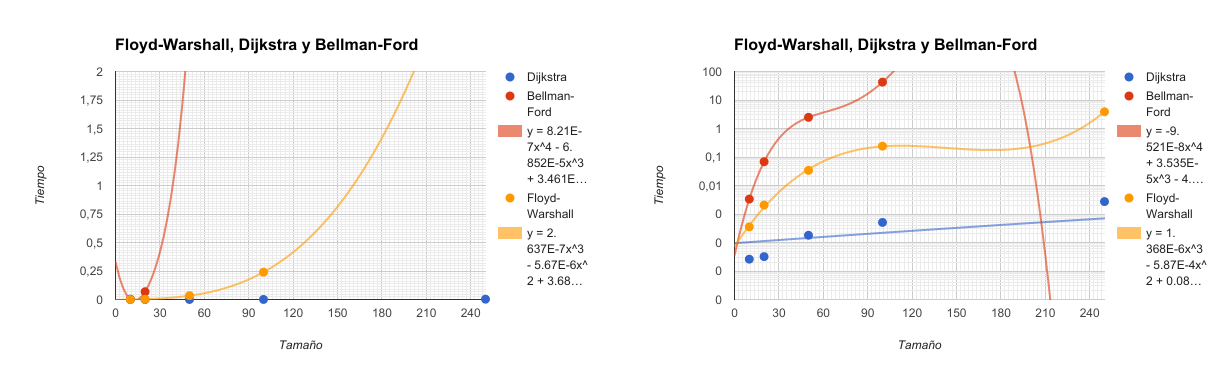
\includegraphics[scale=0.4]{images/grafico-fw-bf-d-doble.png}
		\caption{Floyd Warshall, Bellman-Ford, Dijkstra.}
		\label{fig:fw-bf-d}
	\end{figure}

	\begin{figure}[!htb]
		\centering
		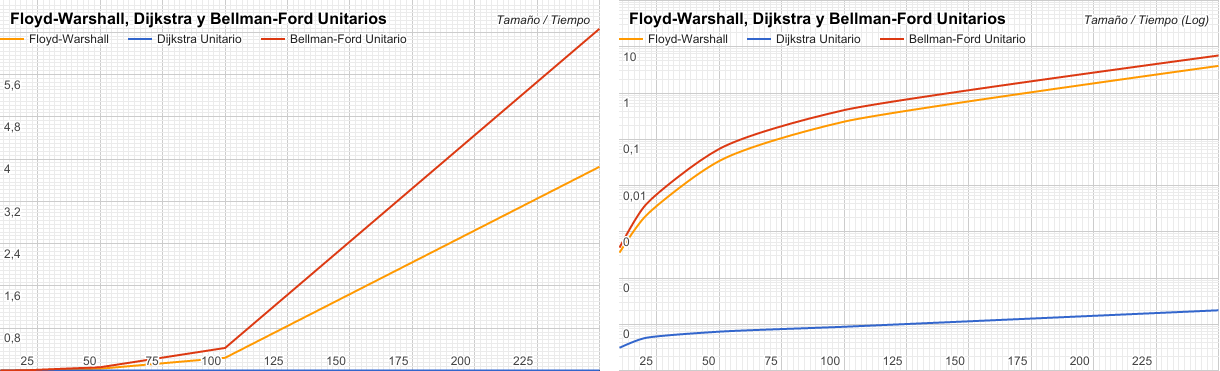
\includegraphics[scale=0.4]{images/grafico-fw-bfu-du-doble.png}
		\caption{Floyd Warshall, Bellman-Ford Unitario, Dijkstra Unitario.}
		\label{fig:fw-bfu-du}
	\end{figure}

\subsection{Cómo correrlo}
	Para correr los algoritmos, desde la carpeta \texttt{src}, correr el comando \texttt{python tiempos.py}.

\pagebreak

\newpage
\section{Código}
\lstset{
	language=Python, columns=flexible, breaklines=true, frame=single, title=bellman\_ford.py
}
\lstinputlisting{../src/bellman_ford.py}

\lstset{ title=creador\_grafos.py }
\lstinputlisting{../src/creador_grafos.py}

\lstset{ title=dijkstra.py }
\lstinputlisting{../src/dijkstra.py}

\lstset{ title=floyd\_warshall.py }
\lstinputlisting{../src/floyd_warshall.py}

\lstset{ title=grafo.py }
\lstinputlisting{../src/grafo.py}

\lstset{ title=parser.py }
\lstinputlisting{../src/parser.py}

\lstset{ title=tiempos.py }
\lstinputlisting{../src/tiempos.py}

\end{document}